\documentclass[
  tucolor,       % remove for less green,
  BCOR=12mm,     % 12mm binding corrections, adjust to fit your binding
  parskip=half,  % new paragraphs start with half line vertical space
  open=any,      % chapters start on both odd and even pages
  cleardoublepage=plain,  % no header/footer on blank pages
  11.5pt,          % font size
]{tudothesis}


%%%%%%%%%%%%%%%%%%%%%%%%%%%%%%%%%%%%%%%%%%%%%%%%%%%%%%%%%%%%%%%%%%%%%%%%%%%%%%%%
%%%%%%%%%%%%%%%%%%   Vorlage für eine Abschlussarbeit   %%%%%%%%%%%%%%%%%%%%%%%%
%%%%%%%%%%%%%%%%%%%%%%%%%%%%%%%%%%%%%%%%%%%%%%%%%%%%%%%%%%%%%%%%%%%%%%%%%%%%%%%%

% Erstellt von Maximilian Nöthe, <maximilian.noethe@tu-dortmund.de>
% ausgelegt für lualatex und Biblatex mit biber

% Kompilieren mit
% latexmk --lualatex --output-directory=build thesis.tex
% oder einfach mit:
% make

\documentclass[
  tucolor,       % remove for less green,
  BCOR=12mm,     % 12mm binding corrections, adjust to fit your binding
  parskip=half,  % new paragraphs start with half line vertical space
  open=any,      % chapters start on both odd and even pages
  cleardoublepage=plain,  % no header/footer on blank pages
]{tudothesis}


% Warning, if another latex run is needed
\usepackage[aux]{rerunfilecheck}

% just list chapters and sections in the toc, not subsections or smaller
\setcounter{tocdepth}{1}

%------------------------------------------------------------------------------
%------------------------------ Fonts, Unicode, Language ----------------------
%------------------------------------------------------------------------------
\usepackage{fontspec}
\defaultfontfeatures{Ligatures=TeX}  % -- becomes en-dash etc.
\setmonofont{Fira Mono}[Scale=MatchLowercase]

% load all used languages
% and set the main language of this thesis
% use this if this thesis is written in German:
% \usepackage[english, ngerman]{babel}
% use this if this thesis is written in English:
\usepackage[ngerman, american]{babel}

% intelligent quotation marks, language and nesting sensitive
\usepackage[autostyle]{csquotes}

% microtypographical features, makes the text look nicer on the small scale
\usepackage{microtype}

%------------------------------------------------------------------------------
%------------------------ Math Packages and settings --------------------------
%------------------------------------------------------------------------------

\usepackage{amsmath}
\usepackage{amssymb}
\usepackage{mathtools}

% Enable Unicode-Math and follow the ISO-Standards for typesetting math
\usepackage[
  math-style=ISO,
  bold-style=ISO,
  sans-style=italic,
  nabla=upright,
  partial=upright,
]{unicode-math}
\setmathfont{Latin Modern Math}
\setmathfont{XITS Math}[range={scr, bfscr}]
\setmathfont{XITS Math}[range={cal, bfcal}, StylisticSet=1]

% nice, small fracs for the text with \sfrac{}{}
\usepackage{xfrac}


%------------------------------------------------------------------------------
%---------------------------- Numbers and Units -------------------------------
%------------------------------------------------------------------------------

\usepackage[
  separate-uncertainty=true,
  per-mode=symbol-or-fraction,
]{siunitx}
\sisetup{math-micro=\text{µ},text-micro=µ}
% automatically choose the right locale
\addto\extrasngerman{\sisetup{locale = DE}}
\addto\extrasenglish{\sisetup{locale = UK}}

%------------------------------------------------------------------------------
%-------------------------------- tables  -------------------------------------
%------------------------------------------------------------------------------

\usepackage{booktabs}       % \toprule, \midrule, \bottomrule, etc

%------------------------------------------------------------------------------
%-------------------------------- graphics -------------------------------------
%------------------------------------------------------------------------------

\usepackage{graphicx, eso-pic}
% currently broken
% \usepackage{grffile}
% \usepackage{titlepic}

% allow figures to be placed in the running text by default:
\usepackage{scrhack}
\usepackage{float}
\floatplacement{figure}{htbp}
\floatplacement{table}{htbp}

% keep figures and tables in the section
\usepackage[section, below]{placeins}

\usepackage{tikz}
\usetikzlibrary{overlay-beamer-styles,calc,tikzmark,decorations.pathreplacing}
\tikzset{fontscale/.style = {font=\relsize{#1}}}
\usepackage{feynman-tikz}


%------------------------------------------------------------------------------
%---------------------- customize list environments ---------------------------
%------------------------------------------------------------------------------

\usepackage{enumitem}

%------------------------------------------------------------------------------
%------------------------------ Bibliographie ---------------------------------
%------------------------------------------------------------------------------

\usepackage[
  backend=biber,   % use modern biber backend
  autolang=hyphen, % load hyphenation rules for if language of bibentry is not
                   % german, has to be loaded with \setotherlanguages
                   % in the references.bib use langid={en} for english sources
]{biblatex}
\addbibresource{references.bib}  % the bib file to use
\DefineBibliographyStrings{german}{andothers = {{et\,al\adddot}}}  % replace u.a. with et al.


\usepackage{pdfpages}
\usepackage{geometry}

% Last packages, do not change order or insert new packages after these ones
\usepackage[pdfusetitle, unicode, hidelinks]{hyperref}
\usepackage{bookmark}
\usepackage[shortcuts]{extdash}
\colorlet{darkRed}{red!80!black}
\colorlet{darkBlue}{blue!70!black}


\renewcommand*{\glstextformat}[1]{\textcolor{black!90}{#1}}


% \renewcommand*{\chapterformat}{\fontsize{48}{48}\color{black}\selectfont\thechapter\autodot\enskip}
% \renewcommand*{\sectionformat}{\makebox[0pt][r]{\thesection\autodot\enskip}}
% \renewcommand*{\subsectionformat}{\makebox[0pt][r]{\thesubsection\autodot\enskip}}

% https://tex.stackexchange.com/questions/330243/chapter-heading-formatting-with-scrreprt
% and from Max Nöthes Ph.D. thesis
\renewcommand\chapterlinesformat[3]{%
  \Ifstr{#1}{chapter}
  {%
    \makebox[\textwidth][l]{%
      \parbox[b]{\textwidth}{\raggedchapter #3}%
      \hspace*{\marginparsep}#2%
    }\\*[-.5\baselineskip]
    \colorrule[tugreen]{\textwidth}{.4pt}%
    \par%
  }
  {\@hangfrom{#2}{#3}}%
}
\interfootnotelinepenalty=10000

\hypersetup{
  pdfa,
  unicode,
  pdfencoding=unicode,
  colorlinks=true,
  linkcolor=tugreen!40!black,
  urlcolor=darkBlue,
  citecolor=black,
}
% Defining a new coordinate system for the page, see
% https://tex.stackexchange.com/questions/89588/positioning-relative-to-page-in-tikz/89592#89592
\makeatletter
\def\parsecomma#1,#2\endparsecomma{\def\page@x{#1}\def\page@y{#2}}
\tikzdeclarecoordinatesystem{page}{
    \parsecomma#1\endparsecomma
    \pgfpointanchor{current page}{north east}
    % Save the upper right corner
    \pgf@xc=\pgf@x%
    \pgf@yc=\pgf@y%
    % save the lower left corner
    \pgfpointanchor{current page}{south west}
    \pgf@xb=\pgf@x%
    \pgf@yb=\pgf@y%
    % Transform to the correct placement
    \pgfmathparse{(\pgf@xc-\pgf@xb)/2.*\page@x+(\pgf@xc+\pgf@xb)/2.}
    \expandafter\pgf@x\expandafter=\pgfmathresult pt
    \pgfmathparse{(\pgf@yc-\pgf@yb)/2.*\page@y+(\pgf@yc+\pgf@yb)/2.}
    \expandafter\pgf@y\expandafter=\pgfmathresult pt
}
\makeatother

% reference for the page coordinate system
% --------------------------
% |(-1,1)    (0,1)    (1,1)|
% |                        |
% |(-1,0)    (0,0)    (1,0)|
% |                        |
% |(-1,-1)   (0,-1)  (1,-1)|
% --------------------------

% ------------------------------------------------------------------------------

% some custom commands
\newcommand{\colorrule}[3][black]{\textcolor{#1}{\rule{#2}{#3}}}
\newcommand{\wip}[2][red]{\textcolor{#1}{\textbf{#2}}}

% renewed commands
\renewcommand*{\glstextformat}[1]{\textcolor{black!70}{\lining #1}}

\renewcommand*{\chapterformat}{\fontsize{48}{48}\color{tugreen}\selectfont\thechapter\autodot\enskip}
\renewcommand*{\sectionformat}{\makebox[0pt][r]{\thesection\autodot\enskip}}
\renewcommand*{\subsectionformat}{\makebox[0pt][r]{\thesubsection\autodot\enskip}}

% metrics
\DeclareMathOperator{\tp}{tp}
\DeclareMathOperator{\fp}{fp}
\DeclareMathOperator{\fn}{fn}
\DeclareMathOperator{\tn}{tn}
\DeclareMathOperator{\recall}{recall}
\DeclareMathOperator{\precision}{precision}
\DeclareMathOperator{\tpr}{tpr}
\DeclareMathOperator{\fpr}{fpr}

% common abbreviations
\NewDocumentCommand \eg {} {e.\,g.\ }
\NewDocumentCommand \ie {} {i.\,e.\ }
\NewDocumentCommand \wrt {} {w.\,r.\,t.\ }

% custom units
\DeclareSIUnit\sigma{σ}
\DeclareSIUnit\pe{\symup{p}.\symup{e}.}

% custom physical quantities
\NewDocumentCommand \Eref {o} {\ensuremath{{E_\text{ref}\IfValueT{#1}{^{#1}}}}}
\NewDocumentCommand \Emax {o} {\ensuremath{{E_\text{max}\IfValueT{#1}{^{#1}}}}}
\NewDocumentCommand \Emin {o} {\ensuremath{{E_\text{min}\IfValueT{#1}{^{#1}}}}}
\NewDocumentCommand \Eest {o} {\ensuremath{{E_\text{est}\IfValueT{#1}{^{#1}}}}}
\NewDocumentCommand \Etrue {o} {\ensuremath{{E_\text{true}\IfValueT{#1}{^{#1}}}}}
\NewDocumentCommand \tobs {o} {\ensuremath{{t_\text{obs}\IfValueT{#1}{^{#1}}}}}
\NewDocumentCommand \Rmax {o} {\ensuremath{{R_\text{max}\IfValueT{#1}{^{#1}}}}}
\NewDocumentCommand \Aeff {o} {\ensuremath{{A_\text{eff}\IfValueT{#1}{^{#1}}}}}
\NewDocumentCommand \pii {o} {\ensuremath{\symup{π}}}

% software names
\NewDocumentCommand \ctapipe {} {\texttt{ctapipe}}
\NewDocumentCommand \numpy {} {\texttt{numpy}}
\NewDocumentCommand \astropy {} {\texttt{astropy}}
\NewDocumentCommand \scipy {} {\texttt{scipy}}
\NewDocumentCommand \sklearn {} {\texttt{sklearn}}

% maths operators
\let\textd\d
\RenewDocumentCommand \d {m} {\TextOrMath{\textd{#1}}{\mathinner{\symup{d}#1}}}

% often named glossary terms
\NewDocumentCommand \cta {} {\gls{cta}}

% cleaning algorithms
\NewDocumentCommand \tailcuts {} {\texttt{TailcutsImageCleaner}}
\NewDocumentCommand \mars {} {\texttt{MARSImageCleaner}}
\NewDocumentCommand \fact {} {\texttt{FACTImageCleaner}}
\NewDocumentCommand \tcc {} {\texttt{TimeConstrainedImageCleaner}}

% cosmic phenomena acronyms
\newacronym{cr}{CR}{cosmic rays}
\newacronym{he}{HE}{high-energy}
\newacronym{hecr}{HECR}{high-energy cosmic ray}
\newacronym{uhecr}{UHECR}{ultra-high-energy cosmic rays}
\newacronym{eas}{EAS}{extensive air shower}
\newacronym{vhe}{VHE}{very-high-energy}
\newacronym{hegr}{HEGR}{high-energy gamma rays}
\newacronym{vhegr}{VHE gamma rays}{very-high-energy gamma rays}
\newacronym{uhegr}{UHEGR}{ultra-high-energy gamma rays}
\newacronym{snr}{SNR}{supernova remnant}
\newacronym[longplural={supernovae}, shortplural={SN}]{sn}{SN}{supernova}
\newacronym[longplural={active galactic nuclei}, shortplural={AGNs}]{agn}{AGN}{active galactic nucleus}
\newacronym{grb}{GRB}{gamma ray burst}
\newacronym{pwn}{PWN}{pulsar wind nebula}
\newacronym{nsb}{NSB}{Night Sky Background}

% CTA acronyms
\newacronym{cta}{CTA}{Cherenkov Telescope Array}
\newacronym{orm}{ORM}{Observatorio del Roque de los Muchachos}
\newacronym[longplural={European Southern Observatorys}, shortplural={ESO}]{eso}{ESO}{European Southern Observatory}
\newacronym{lst}{LST}{Large-Sized Telescope}
\newacronym{mst}{MST}{Medium-Sized Telescope}
\newacronym{sst}{SST}{Small-Sized Telescope}

% IACT and tech acronyms
\newacronym{iact}{IACT}{Imaging Air Cherenkov Telescope}
\newacronym{pmt}{PMT}{photo multiplier tube}
\newacronym{sipm}{SiPM}{silicon photomultiplier}

% other experiments
\newacronym{magic}{MAGIC}{Major Atmospheric Gamma-Ray Imaging Cherenkov}
\newacronym{veritas}{VERITAS}{Very Energetic Radiation Imaging Telescope Array System}
\newacronym{hess}{H.\,E.\,S.\,S.}{High Energy Stereoscopic System}
\newacronym{fermilat}{\textit{Fermi}-LAT}{\textit{Fermi} Large Area Telescope}

% software and IT
\newacronym{mc}{MC}{Monte Carlo}
\newacronym{corsika}{\texttt{CORSIKA}}{Cosmic Ray Simulations for Kascade}

% math, metrics etc.
\newacronym{roc}{ROC}{Receiver Operating Characteristic}
\newacronym{auc}{AUC}{Area Under the Curve}
\newacronym{tpr}{tpr}{True Positive Rate}
\newacronym{fpr}{fpr}{False Positive Rate}
\newacronym{tnr}{tnr}{True Negative Rate}
\newacronym{fnr}{fnr}{False Negative Rate}
\newacronym{ppv}{ppv}{Positive Predictive Value}
\newacronym{acc}{acc}{Accuracy}
\newacronym{ba}{ba}{Balanced Accuracy}



\input{bib-settings.tex}

\author{Anno Knierim}
\title{Finding optimal hyperparameters for cleaning algorithms for the Cherenkov Telescope Array}
\date{2022}
\birthplace{Hagen}
\chair{Chair of Experimental Physics V}
\division{Department of Physics}
\thesisclass{Bachelor of Science}
\submissiondate{7 September 2022}
\firstcorrector{Prof.~Dr.~Dr.~Wolfgang Rhode}
\secondcorrector{Dr.~Dirk Wiedner}


\begin{document}
\frontmatter

\AddToShipoutPictureBG*{%
  \AtTextLowerLeft{%
    \makebox[\textwidth]{%
      \ifdefined\lsttitle
        \raisebox{\dimexpr\textheight-\height}{\tikz[remember picture,overlay] \node[opacity=0.3,inner sep=15pt] at (current page.center){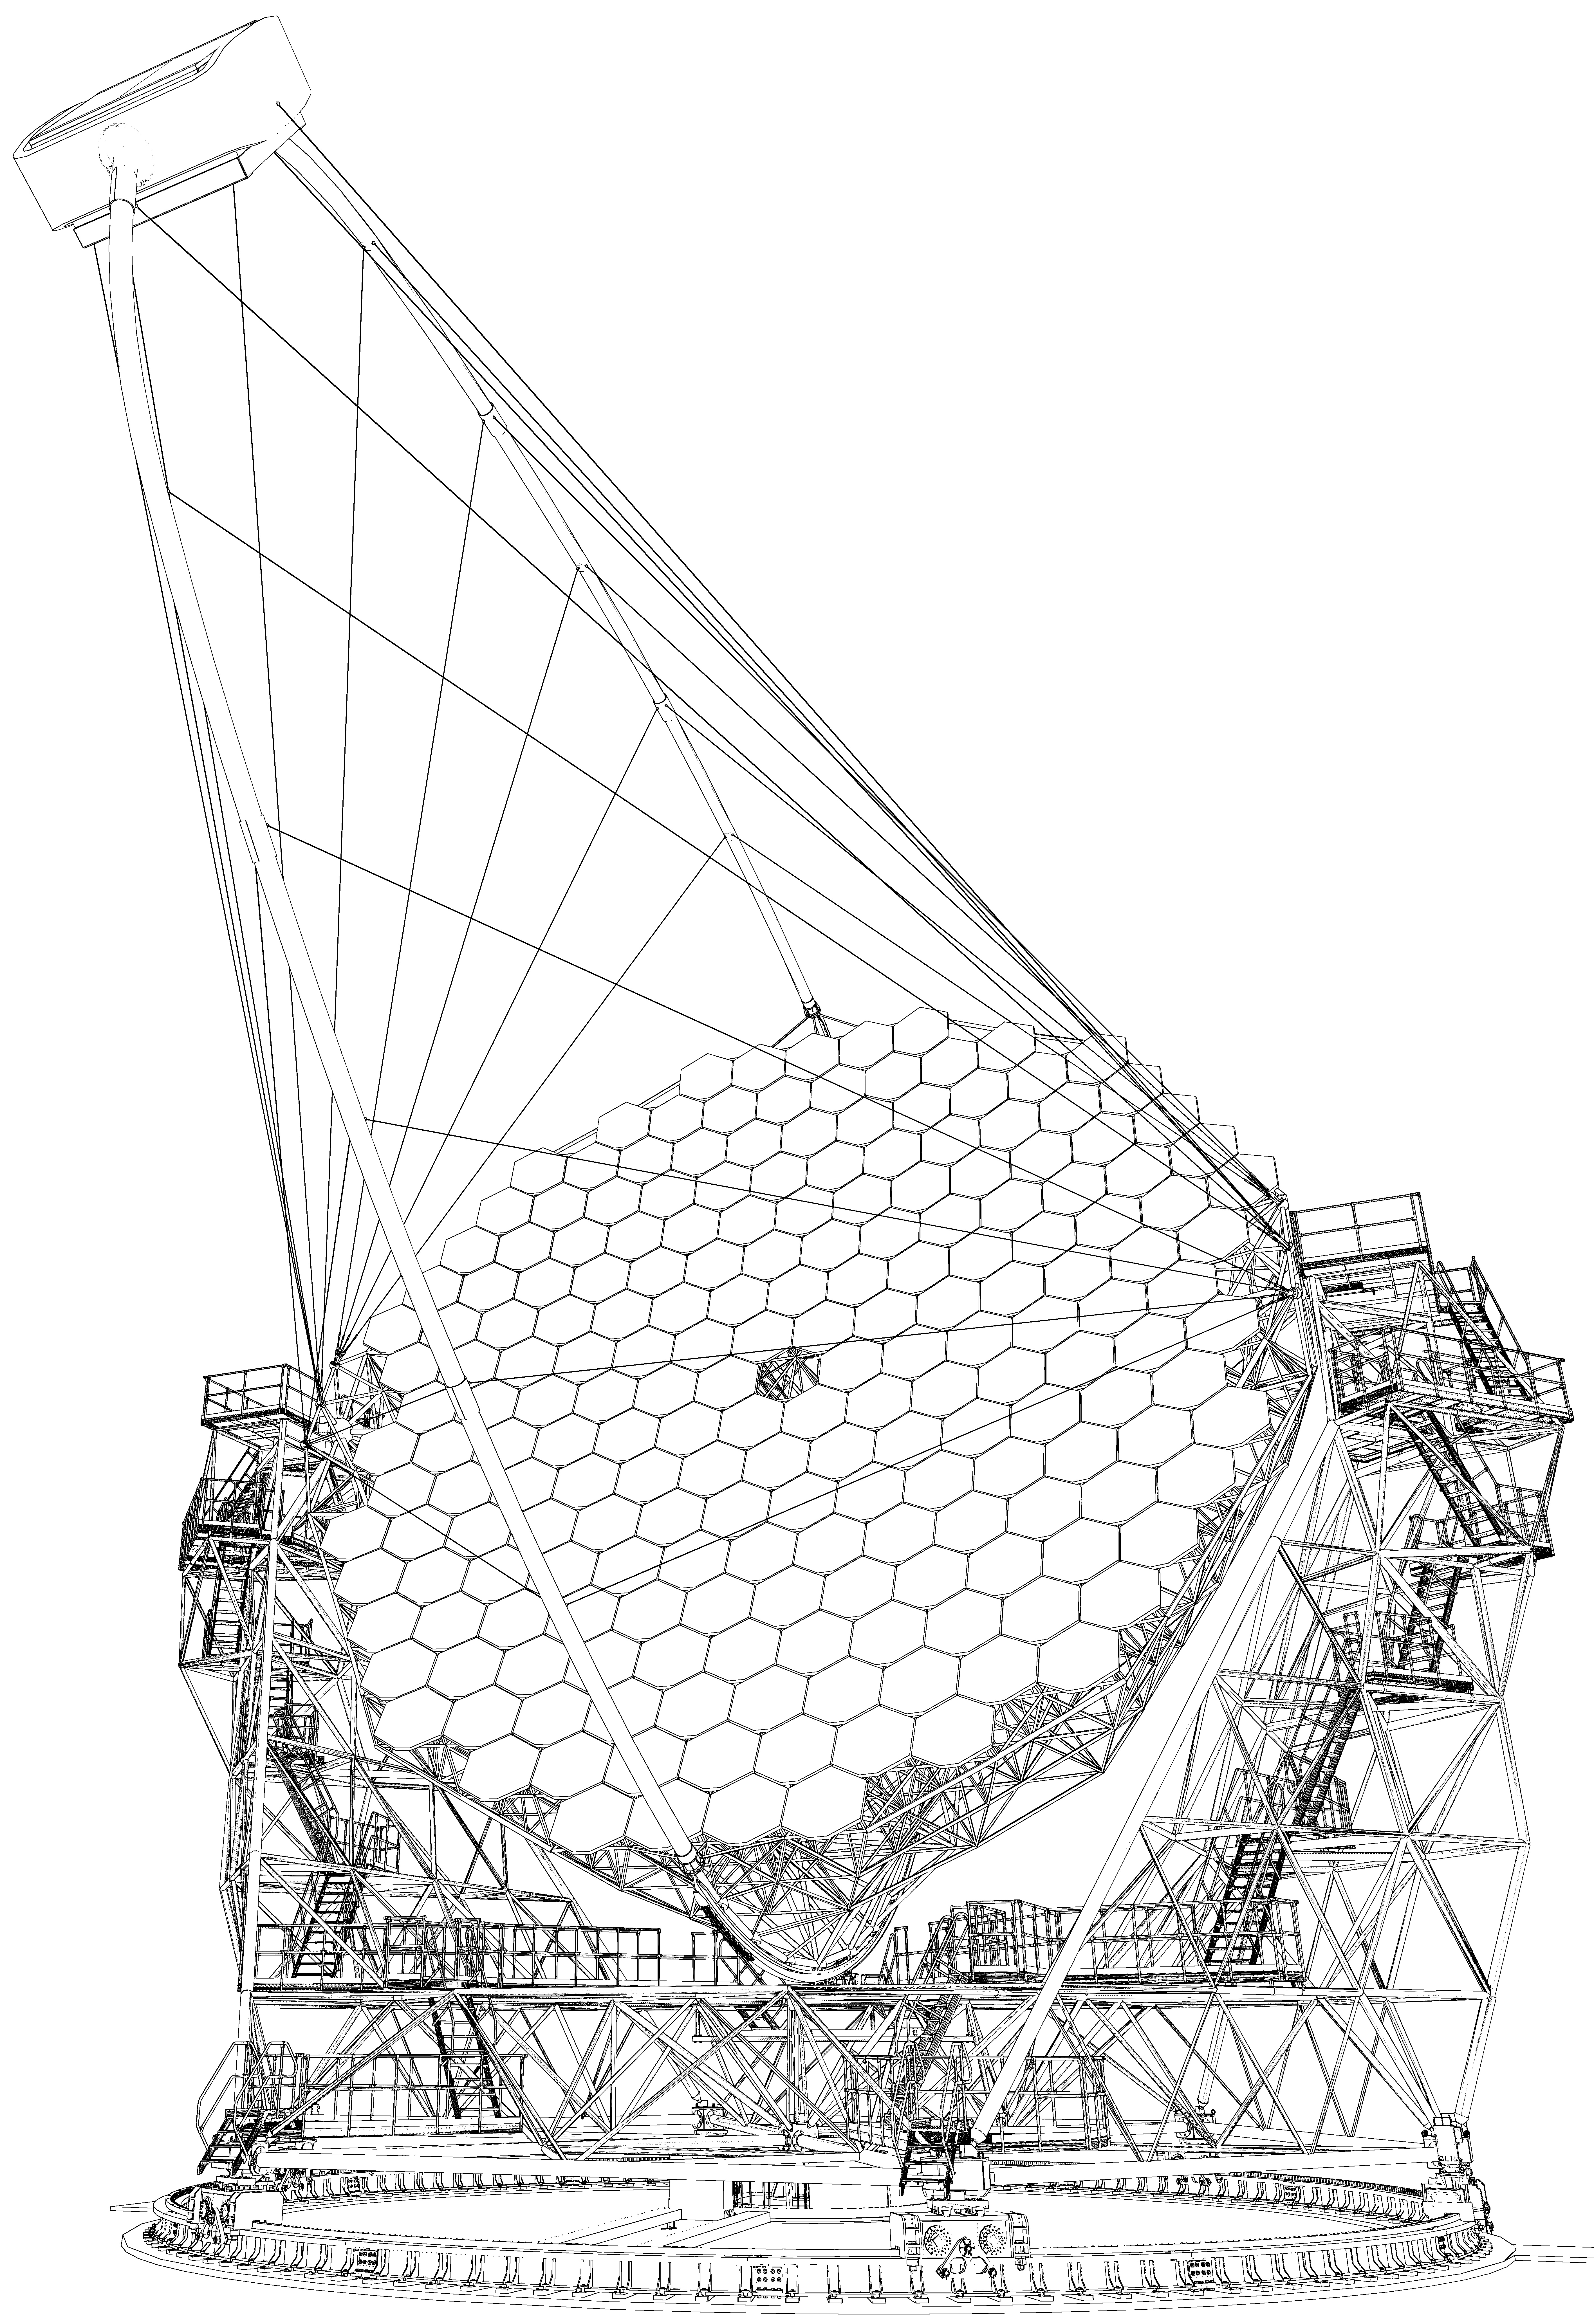
\includegraphics[width=0.94\paperwidth,height=0.94\paperheight]{graphics/contours_lst.jpg}};}%
        \raisebox{\dimexpr\textheight-\height}{\tikz[remember picture,overlay] \node[inner sep=15pt, anchor=north east] at (current page.north east){\hspace{-15em}\includegraphics[width=0.4\paperwidth]{logos/tu-logo.pdf}};}%
      \else
        \raisebox{\dimexpr\textheight-\height}{\tikz[remember picture,overlay] \node[opacity=0.25,inner sep=15pt] at (current page.center){\includegraphics[width=0.94\paperwidth,height=0.94\paperheight]{graphics/contours_mst.jpg}};}%
        \raisebox{\dimexpr\textheight-\height}{\tikz[remember picture,overlay] \node[inner sep=15pt, anchor=north west] at (current page.north west){\includegraphics[width=0.4\paperwidth]{logos/tu-logo.pdf}};}%
      \fi%
    }%
  }%
}
\maketitle

% Corrector page
\makecorrectorpage

% abstract
% \thispagestyle{plain}

\section*{Abstract}
In recent years, gamma astronomy has become a vastly studied field of astrophysics.
Since then, many \gls{iact} experiments have been producing insights into sources of
high-energy gamma-rays. Continuing this trend, the \gls{cta}, a next-generation \gls{iact},
will provide new data targeting some of the highest energies of the gamma-ray spectrum.

In this thesis, I consider the four cleaning algorithms implemented in the low-level data processing software \ctapipe{},
currently developed for \gls{cta}. Furthermore, I will determine optimized hyperparameters for each algorithm
with the aim of improving their performance. A grid search achieves this objective
over a range of reasonable hyperparameters. The data used in this work is diffuse gamma \gls{mc} simulation data for
the \glspl{mst} at the northern site of \cta{} on the Canarian island of La Palma.

The hyperparameters determined for the \tcc{} algorithm in \ctapipe{} improve its performance over
its default parameters significantly \wrt the angular resolution, while the other algorithms are only
slightly improved by the respective hyperparameters or their results are not improved at all.
In terms of metrics, the performance of the \tcc{} algorithm only improved slightly with the new parameters, while \fact{}
performed worse than with its default values. Overall, however, \fact{} performed better than the other
algorithms.


\section*{Kurzfassung}
\begin{otherlanguage}{ngerman}
In den vergangenen Jahrzehnten hat sich die Gammaastronomie zu einem viel erforschten Bereich der
Astrophysik entwickelt. Seitdem haben bildgebende, atmosphärische Tscherenkow-Teleskope (\gls{iact})
zahlreiche neue Erkenntnisse im Bereich der hochenergetischen Gammastrahlen und deren Quellen geliefert.
Mit \gls{cta}, einem \gls{iact} der nächsten Generation, werden neue Daten in einigen der höchsten
Energiebereiche der Gammastrahlen erwartet.

In dieser Arbeit betrachte ich die vier Bildreinigungsalgorithmen an, die in Software \ctapipe{} implementiert
sind, welche sich zur Zeit für \cta{} in Entwicklung befindet. Zudem bestimme ich optimierte
Hyperparameter für jeden Algorithmus mit dem Ziel, die Leitung der Bildreinigungsalgorithmen zu verbessern.
Dies wird mittels einer Grid-Search über eine Auswahl von Hyperparametern durchgeführt. Die zu diesem
Zweck verwendeten Daten bestehen aus diffusen Gammadaten, die mittels einer \gls{mc}-Simulation für die
\glspl{mst} des nördlichen Standorts \gls{cta}s auf der Kanarischen Insel La Palma erzeugt wurden.

Die Ergebnisse zeigen, dass die in dieser Arbeit gefundenen Hyperparameter die Leistung des \tcc{}-Algorithmus
in Bezug auf die Winkelauflösung verbesserten, während die Leistungen der anderen Algorithmen nur wenig
verbessert wurden oder gleiche Ergebnisse lieferten, wie mit den Standardparametern.
In Bezug auf die Metriken konnten die gefundenen Hyperparameter bei \tcc{} eine leichte Verbesserung
bewirken, während die Parameter bei \fact{} sogar eine etwas schlechtere Leistung bewirkten.
Insgesamt lieferte \fact{} allerdings bessere Ergebnisse als die anderen Algorithmen.
\end{otherlanguage}
\glsresetall
% \listoftodos

{\hypersetup{hidelinks}
\tableofcontents
}


\mainmatter
\chapter{Gamma-Ray Astronomy}
\label{ch:gamma-ray-astronomy}

Astronomy, being one of the oldest sciences, is a vast field of study dating back to the Babylonians.
From the earliest days of civilization, astronomers have been studying the stars and the planets to
understand the universe. It, therefore, is no surprise that astronomy spawned a great number of discoveries
throughout the centuries. Whereas first observations were made by eye only, we now have access to a multitude
of experiments and telescopes that deepen our understanding of the universe. With the discovery of
\gls{cr} by Victor Hess in the early 20th century, the new field of astroparticle physics was born \cite{longair1981}.

From then on we found many different types of cosmic messengers, the most recent being the discovery of
gravitational waves in 2015 \cite{PhysRevLett.116.061102}.\todo{rewrite this (maybe)}

\begin{figure}
    \centering
    \includegraphics[width=0.8\textwidth]{graphics/figure5.png}
    \caption{Different types of cosmic rays on their way to Earth. Charged particles like protons and electrons
    are deflected by magnetic fields and therefore making it hard to pinpoint the source. Only the
    origin of photons and neutrinos can be reconstructed directly since they are uncharged particles
    and therefore travel in straight lines. However, photons can be absorbed or created in multiple
    mechanisms. Since neutrinos only rarely interact with matter via the weak force, their detection
    is significantly harder than for photons \cite{fig5}.}
    \label{fig:fig5}
\end{figure}

\gls{cr} come in different types, that are either charged or uncharged, as shown in \autoref{fig:fig5}.
Charged particles like electrons, protons or atomic nuclei are difficult to trace back to their origin
as they are deflected by the cosmic electromagnetic fields. Uncharged particles like photons or
neutrinos, however, travel in straight lines, making it easier to reconstruct their origins,
although photons can be absorbed by dust clouds in their way.

Since neutrinos are harder to detect due to their weak interaction with matter, photons are easier to study
with space- and ground-based experiments.

Therefore, in recent years, gamma-ray astronomy has become an important research field in astroparticle physics.
The term gamma-rays is generally denoted as photons with energies above \SI{100}{\kilo\eV}
\cite{funk}. Due to this high-energy nature, gamma rays pose some of the most powerful \gls{cr} in
the universe and since photons at such energies cannot be produced by thermal processes, their origin
can be described by higher order processes involving charged particles. Sources for gamma rays include
\glspl{snr}, Pulsars, Blazars, \glspl{agn} or \glspl{grb}.

\begin{description}
    \item [\glspl{snr}] are the remnants of a supernova explosion.
    \item [Pulsars] are rotating neutron stars that emit gamma rays in the form of pulsations.
    \item [Blazars] are \glspl{agn} that are highly variable and emit gamma rays in the form of
    flares.
    \item [\glspl{agn}] are active galactic nuclei that emit gamma rays in the form of flares.
    \item [\glspl{grb}] are gamma-ray bursts that are the most energetic explosions in the universe.
\end{description}

\begin{figure}
    \centering
    \includegraphics[width=0.8\textwidth]{build/fermi_catalog.pdf}
    \caption{Hammer projection of the Fermi-LAT 4FGL catalog data of gamma-ray sources. The skymap
    shows the flux of gamma-ray sources in \(\si{\tera\eV\per\centi\meter\squared\per\second}\)
    over a span of \(\num{10}\) years \cite{fermi4fgl}.}
    \label{fig:fermilat}
\end{figure}
Gamma rays can be detected by a variety of experiments, either ground- or space-based. Space-based
experiments like the \gls{fermilat} are usually more sensitive to lower energies, whereas ground-based experiments are more
sensitive to higher energies. The \gls{fermilat} is a space-based gamma-ray observatory that was launched
in 2008 and is still in operation today. \autoref{fig:fermilat} shows the gamma-ray sky as observed by the
\gls{fermilat} over a span of \(\num{10}\) years.

For the past two decades, ground-based \gls{iact} experiments like the \gls{magic} telescopes, the
\gls{veritas} and the \gls{hess} have been monitoring these \gls{vhegr} to gain an understanding of
their production. This allowed us to determine different source classes inside and outside our galaxy,
with the most important source class inside our galaxy being \glspl{snr} such as the Crab Nebula.






\chapter{IACTs and the Cherenkov Telescope Array}

Most modern gamma-ray observations are performed with \glspl{iact}, which are ground-based telescopes
or arrays of telescopes that use the Cherenkov light emitted by \gls{eas} in the atmosphere.
Since they are ground-based, \glspl{iact} are taking advantage of the Earth's atmosphere to get a larger
effective area than space-based instruments. This is especially true for energies above \SI{100}{\giga\eV},
\todo{confirm values} where the gamma-ray flux is low compared to lower energies. The cosmic ray flux
is shown in \autoref{fig:flux}.

% \begin{figure}
%     \centering
%     \input{build/cosmic_rays.pgf}
%     \caption{The cosmic ray flux as a function of energy. The flux is given in \si{\per\second\per\square\meter\per\steradian}.}
%     \label{fig:flux}
% \end{figure}
% \todo{PLACEHOLDER, MAYBE USE A DIFFERENT PLOT?}

The \cta{} is a new generation of \glspl{iact} that will consist of two sites,
one of which will be built at the \gls{orm} on the Canarian island of La Palma while the other site
will be built in the southern hemisphere at the \glspl{eso} Paranal Observatory in the Atacama desert
of northern Chile.

\begin{figure}
    \centering
    \includegraphics[width=\textwidth]{graphics/cherenkov_radiation.pdf}
    \caption{}
    \label{fig:cherenkov}
\end{figure}
\chapter{Data processing with \ctapipe{}}
\label{ch:data-processing}

The analysis in this work was done with the open-source low-level data processing software for \cta{},
\ctapipe{} \cite{ctapipe}, specifically version \texttt{0.15.1}.
% The version used is the development version \texttt{0.15.1.dev166+gf26107f},
% henceforth shortened to version \texttt{0.15.1}.
The goal of \ctapipe{} is to provide a complete analysis
framework ranging from data calibration and image extraction to the reconstruction of events and the
analysis of their properties. In this chapter, I will first describe how the data
were simulated in \autoref{sec:data-simulation} and then, in \autoref{sec:data-levels}, explain the different
data levels and \ctapipe{}'s various analysis steps. In \autoref{sec:pipeline} I will
explain the full pipeline created for this work.


\section{Data simulation}
\label{sec:data-simulation}

In its current in-development state, \ctapipe{} is used and tested with simulated data, as the software
can only be sufficiently tested when the output is compared to truth data. This data is created with the help of
\gls{mc} simulations. The software used for these simulations is called \gls{corsika} \cite{corsika} and
allows for detailed simulation of \glspl{eas} initiated by \glspl{hecr}. The showers are observed by
a virtual \gls{iact} array, the \texttt{sim\_telarray} \cite{bernlohr2008}. The resulting so-called
\texttt{simtel} data is used in \ctapipe{} and can be processed as described in \autoref{sec:data-levels}
and \autoref{fig:ctapipe}. Some of the data properties are listed in \autoref{tab:simtel}.

This data is the basis for the analysis in this work. A total of
\(\num{20}\) \texttt{simtel} runs of diffuse gamma data were used for the initial analysis, \ie the
testing of different parameters as described in \autoref{sec:hyperparameters}. The individual runs
were processed into \dlo{} files and merged before being processed for each cleaning setting.

Once promising settings are found, a larger dataset containing \(\num{987}\) runs is processed with these
selected settings, allowing for more statistics and a better comparison of the cleaning algorithms.

\begin{table}
    \centering
    \caption{Simtel data properties of the \gls{corsika} simulation used for the datasets in this works
    analysis.}
    \label{tab:simtel}
    \rowcolors{0}{white!92!black}{}
    \begin{tabular}{l r}
        \hiderowcolors
        & Diffuse Gamma data \\
        \showrowcolors
        {Energy range / \si{\tera\eV}} & \numrange[range-phrase={--}]{0.003}{330} \\
        {Zenith angle / \si{\degree}} & \num{20} \\
        {View cone angle / \si{\degree}} & \num{10} \\
        {Number of showers} & \num{50000} \\
        {Spectral index} & \num{-2.0} \\
        {Maximum scatter range / \si{\meter}} & \num{1900} \\
    \end{tabular}
\end{table}


\section{Data Levels in \ctapipe{}}
\label{sec:data-levels}

There are several data levels in \ctapipe{}, spanning from the raw data \rzero{} to the reconstructed events
\dlt{}, with the raw data levels being denoted by an \textbf{R} and the calibrated data levels by a \textbf{D}.
\autoref{fig:ctapipe} shows a simplified overview of the data levels and the analysis steps.
The raw data level \rzero{} is the data that comes directly from the photodetectors. The time-resolved
signal of the data is calibrated from \rzero{} to \rone{}. Then the data volume gets reduced
(\rone{} \rightarrow \dlz{}) by a selection of waveforms.

The \dlz{} data level is the first level being stored and also the first level to be processed from
the simulation datasets used in this work. From \dlz{} to \dloa{}, the images of the data are extracted
from the time pulses, which are then cleaned by a cleaning algorithm, allowing for parametrization
of the events (\dloa{} \rightarrow \dlob{}). The parametrized events can then be reconstructed
(\dlob{} \rightarrow \dlt{}) and stored on the \dlt{} data level.

\begin{figure}
    \centering
    \includegraphics[width=\textwidth]{graphics/ctapipe.png}
    \caption{Data levels in \ctapipe{}. Raw data levels are denoted by an \textbf{R} and calibrated
    data levels by a \textbf{D}. The raw data first gets calibrated (\rzero{} \rightarrow \rone{})
    and then reduced in volume by selecting waveforms (\rone{} \rightarrow \dlz{}). From there the
    images are extracted (\dlz{} \rightarrow \dloa{}) and cleaned with a cleaning algorithm. This
    allows for parametrization of the events (\dloa{} \rightarrow \dlob{}). The parametrized events
    can then be reconstructed (\dlob{} \rightarrow \dlt{}) \cite{noethe_thesis, hackfeld}.}
    \label{fig:ctapipe}
\end{figure}

\section{This work's data processing pipeline}
\label{sec:pipeline}
In this work, the data processing pipeline is as follows: First, several simulation data runs are
selected and processed with \ctapipe{}. Then, the datasets are merged and serve as a basis for a re-run
of the combined dataset with various parameter combinations described in \autoref{ch:finding-hyperparams}.

The settings for \ctapipe{} are saved in two configuration files: First, a file, that sets up the
cleaning process and what data to write to the output file. For the preprocessing step of this work's
pipeline, the cleaning settings are not relevant, as this step only serves to create a merged dataset.
The second file contains a list of all the allowed telescope IDs. This allows a selection of the telescopes
that are used in the analysis. This is especially helpful if one wants to only analyze \gls{mst}-related
data, like in this work.

For the re-run of the combined dataset, the cleaning settings are used\footnote{As opposed to the preprocessing step},
however, as this step is the heart of this work's search for the optimal hyperparameters.
The configuration files used are shown in \hyperref[ap:config_files]{appendix \ref{ap:config_files}}.

Each resulting dataset can then be processed on an array or telescope data level, resulting in
\dloa{} image plots, values for the angular resolution and the efficiency as well as metrics for the
performance. An in-detail description of how this helps to compare the performance of the different
cleaning algorithms can be found in \autoref{sec:hyperparameters}. A schematic overview of the data
processing pipeline of this work is shown in \autoref{fig:data-processing}.

\begin{figure}
    \centering
    \includegraphics[width=\textwidth]{graphics/data_pipeline.pdf}
    \caption{Schematic overview of the data pipeline used for this work. Single runs of the simulation
    data are processed with \ctapipe\texttt{-process} and then merged via the tool \ctapipe\texttt{-merge} (green shaded area).
    The merged data is then processed on the array or telescope data level resulting in scores for metrics
    as well as \dlo{} \texttt{images} and plots for the angular resolution and the effective area (blue shaded area).}
    \label{fig:data-processing}
\end{figure}



\chapter{Finding Optimal Hyperparameters for the Cleaning Algorithms}
\label{ch:finding-hyperparams}

This work aims to find optimal hyperparameters for the cleaning algorithms used in \ctapipe{}.
Optimizing the cleaning step of the \dlo{} data level in \autoref{sec:data-levels} can most certainly lead to a better
reconstruction of the events in a dataset. Therefore, a tweaking of the available parameters of each
cleaner is necessary. In this chapter, I will first introduce the cleaning algorithms and their parameters
in \autoref{sec:cleaning-algorithms} and then describe the procedure to find optimal hyperparameters
in \autoref{sec:hyperparameters}.

\section{Cleaning Algorithms}
\label{sec:cleaning-algorithms}

Version \texttt{0.15.1} of \ctapipe{} features four cleaning algorithms, two of which are time-based.
The \tailcuts{} algorithm is the most basic algorithm of the four and serves as a good
starting point for the development of new cleaning algorithms. Its first step is to select all
pixels that are above a certain threshold, the \texttt{picture} or \texttt{core\_threshold}. These
pixels are the core part of the signal and are the brightest. The \tailcuts{} algorithm
then selects all pixels that are above the so-called \texttt{boundary\_threshold} and are neighboring
the core pixels. A visualization of the algorithm is shown in \autoref{fig:tailcuts_clean} for the
default values of the algorithm.

\begin{figure}
    \centering
    \begin{subfigure}[t]{0.33\textwidth}
        \includegraphics[width=\textwidth]{plots/cleaner_steps/tail_1.pdf}
    \end{subfigure}
    \begin{subfigure}[t]{0.33\textwidth}
        \includegraphics[width=\textwidth]{plots/cleaner_steps/tail_2.pdf}
    \end{subfigure}
    \caption{Visualization of the \tailcuts{} algorithm for a \gls{mst} NectarCam image. First, all
    pixels above the \texttt{core\_threshold} are selected. Then, all pixels neighboring the core
    pixels that are above the \texttt{boundary\_threshold} are selected.}
    \label{fig:tailcuts_clean}
\end{figure}

The \mars{} algorithm is very much based on the \tailcuts{}
algorithm and features an additional step, in that it also selects all neighbors of a neighbor of a
core pixel, if they are above the \texttt{boundary\_threshold}. The three steps for the \mars{} algorithm
are shown in \autoref{fig:mars_cleaning} for the default values of the algorithm.

\begin{figure}
    \centering
    \begin{subfigure}[t]{0.32\textwidth}
        \includegraphics[width=\textwidth]{plots/cleaner_steps/mars_1.pdf}
    \end{subfigure}
    \hfill
    \begin{subfigure}[t]{0.32\textwidth}
        \includegraphics[width=\textwidth]{plots/cleaner_steps/mars_2.pdf}
    \end{subfigure}
    \hfill
    \begin{subfigure}[t]{0.32\textwidth}
        \includegraphics[width=\textwidth]{plots/cleaner_steps/mars_3.pdf}
    \end{subfigure}
    \caption{Visualization of the \mars{} algorithm for a \gls{mst} NectarCam image. The first two
    steps are identical to the \tailcuts{} algorithm. The third step selects all neighbors of a neighbor of a
    core pixel, if they are above the \texttt{boundary\_threshold}.}
    \label{fig:mars_cleaning}
\end{figure}

\begin{figure}
    \centering
    \begin{subfigure}[t]{0.32\textwidth}
        \includegraphics[width=\textwidth]{plots/cleaner_steps/fact_1.pdf}
    \end{subfigure}
    \hfill
    \begin{subfigure}[t]{0.32\textwidth}
        \includegraphics[width=\textwidth]{plots/cleaner_steps/fact_2.pdf}
    \end{subfigure}
    \hfill
    \begin{subfigure}[t]{0.32\textwidth}
        \includegraphics[width=\textwidth]{plots/cleaner_steps/fact_3.pdf}
    \end{subfigure}
    \begin{subfigure}[b]{0.32\textwidth}
        \includegraphics[width=\textwidth]{plots/cleaner_steps/fact_4.pdf}
    \end{subfigure}
    \hfill
    \begin{subfigure}[b]{0.32\textwidth}
        \includegraphics[width=\textwidth]{plots/cleaner_steps/fact_5.pdf}
    \end{subfigure}
    \hfill
    \begin{subfigure}[b]{0.32\textwidth}
        \includegraphics[width=\textwidth]{plots/cleaner_steps/fact_6.pdf}
    \end{subfigure}
    \caption{Visualization of the \fact{} algorithm for a \gls{mst} NectarCam image. The first
    step selects all pixels above the \texttt{core\_threshold}. The second step removes all pixels that have less than
    \(N\) neighbors. The third step selects all pixels neighboring the remaining pixels that are above the
    \texttt{boundary\_threshold}. The fourth step removes all pixels that have less than \(N\) neighbors,
    that have arrived within a given timeframe. The fifth and sixth steps are analogous to steps two and four.}
    \label{fig:fact_cleaning}
\end{figure}

The \fact{} algorithm is a time-based cleaning algorithm that first selects all pixels that are above
the \texttt{core\_threshold}. Then, all pixels that have less than \(N\) neighbors are removed. The
\texttt{min\_number\_neighbors} parameter is set to \(\num{2}\) by default. For the third step, all pixels neighboring
the remaining pixels that are above the \texttt{boundary\_threshold} are selected. After that, all
pixels that have less than \(N\) neighbors and that have arrived within a given timeframe are removed.
The \texttt{time\_limit} parameter is set to \(\SI{5}{\nano\second}\) by default. Again, all pixels
with less than \(N\) neighbors are removed. The last step once again removes pixels with less than
\(N\) neighbors, arriving within the given time limit. The visualization of the algorithm is shown in
\autoref{fig:fact_cleaning} for the default values of the algorithm.

The \tcc{} algorithm is another time-based algorithm, coming from the \gls{magic} collaboration.
It first selects all pixels that are above the \texttt{core\_threshold}. Then, all pixels that have
less than \(N\) neighbors are removed. The \texttt{min\_number\_neighbors} parameter is set to \(\num{1}\) by default.
After that, all core pixels whose arrival times are within a given timeframe of the average arrival time.
This \texttt{time\_limit\_core} parameter is set to \(\SI{4.5}{\nano\second}\) by default. As a fourth step,
the \tcc{} algorithm finds all pixels above the \texttt{boundary\_threshold}. Then, all pixels with
less than \(N\) neighbors arriving within a given timeframe are removed. This \texttt{time\_limit\_boundary}
parameter is set to \(\SI{1.5}{\nano\second}\) by default. The visualization of the algorithm is shown in
\autoref{fig:tcc_cleaning} for the default values of the algorithm.

\begin{figure}
    \centering
    \begin{subfigure}[t]{0.32\textwidth}
        \includegraphics[width=\textwidth]{plots/cleaner_steps/tcc_1.pdf}
    \end{subfigure}
    \hfill
    \begin{subfigure}[t]{0.32\textwidth}
        \includegraphics[width=\textwidth]{plots/cleaner_steps/tcc_2.pdf}
    \end{subfigure}
    \hfill
    \begin{subfigure}[t]{0.32\textwidth}
        \includegraphics[width=\textwidth]{plots/cleaner_steps/tcc_3.pdf}
    \end{subfigure}
    \begin{subfigure}[]{0.32\textwidth}
        \includegraphics[width=\textwidth]{plots/cleaner_steps/tcc_4.pdf}
    \end{subfigure}
    \begin{subfigure}[]{0.32\textwidth}
        \includegraphics[width=\textwidth]{plots/cleaner_steps/tcc_5.pdf}
    \end{subfigure}
    \caption{Visualization of the \tcc{} algorithm for a \gls{mst} NectarCam image. The first step
    selects all pixels above the \texttt{core\_threshold}. The second step removes all pixels that have less than
    \(N\) neighbors. The third step selects all pixels whose arrival times are within a given timeframe of the
    \texttt{time\_limit\_core} parameter. The fourth step selects all pixels above the \texttt{boundary\_threshold}.
    The fifth step removes all pixels with less than \(N\) neighbors, that have arrived within a given timeframe
    of the \texttt{time\_limit\_boundary} parameter.}
    \label{fig:tcc_cleaning}
\end{figure}
\vspace{-0.5cm}
\section{Hyperparameters}
\label{sec:hyperparameters}

The hyperparameters of each cleaning algorithm are set in a specific \texttt{configuration} file. There,
the user can set and change the parameters, shown in \autoref{tab:hyperparameters}. \tailcuts{}
and \mars{} can be set-up with only three parameters: the \texttt{picture\_threshold}, the
\texttt{boundary\_threshold} and \texttt{min\_number\_picture\_neighbors}. The time-based algorithms
have additional parameters: First of all a \texttt{time\_limit} for \fact{} and then a \texttt{time\_limit\_core} as
well as a \texttt{time\_limit\_boundary} for \tcc{}.
\begin{table}
    \centering
    \caption{The four cleaning algorithms and their hyperparameters. Being the most basic algorithms,
    \tailcuts{} and \mars{} have only three parameters, while the \fact{} and \tcc{} algorithms have
    one and two additional time-based parameters, respectively. This table shows the default values
    and, if the parameters have them, also their units, as they are implemented in the \ctapipe{}
    source code for version \texttt{0.15.1}.}
    \label{tab:hyperparameters}
    \rowcolors{0}{white!92!black}{}
    \adjustbox{varwidth=\linewidth,scale=0.9}{%
    \begin{tabular}{l l l}
        \hiderowcolors
        \textbf{Cleaning Algorithm} & \textbf{Hyperparameter} & \textbf{Default Values} \\
        \showrowcolors
        \tailcuts{} & \texttt{picture\_threshold}               & \qquad\(\SI{7}{\pe}\) \\
                    & \texttt{boundary\_threshold}              & \qquad\(\SI{5}{\pe}\) \\
                    & \texttt{min\_number\_picture\_neighbors}  & \qquad\(\num{0}\) \\
        \addlinespace[0.5em]
        \mars{}     & \texttt{picture\_threshold}               & \qquad\(\SI{7}{\pe}\) \\
                    & \texttt{boundary\_threshold}              & \qquad\(\SI{5}{\pe}\) \\
                    & \texttt{min\_number\_picture\_neighbors}  & \qquad\(\num{0}\) \\
        \addlinespace[0.5em]
        \fact{}     & \texttt{picture\_threshold}               & \qquad\(\SI{4}{\pe}\) \\
                    & \texttt{boundary\_threshold}              & \qquad\(\SI{2}{\pe}\) \\
                    & \texttt{time\_limit}                      & \qquad\(\SI{5}{\nano\second}\) \\
                    & \texttt{min\_number\_picture\_neighbors}  & \qquad\(\num{2}\) \\
        \addlinespace[0.5em]
        \tcc{}      & \texttt{picture\_threshold}               & \qquad\(\SI{7}{\pe}\) \\
                    & \texttt{boundary\_threshold}              & \qquad\(\SI{5}{\pe}\) \\
                    & \texttt{time\_limit\_core}                & \qquad\(\SI{4.5}{\nano\second}\) \\
                    & \texttt{time\_limit\_boundary}            & \qquad\(\SI{1.5}{\nano\second}\) \\
                    & \texttt{min\_number\_picture\_neighbors}  & \qquad\(\num{1}\) \\
  \end{tabular}}
\end{table}
The full configuration files for the default settings of each cleaning algorithm are listed in
\hyperref[ap:config_files]{appendix \ref{ap:config_files}}. There, one can also find the configuration files for the allowed telescopes
as described in \todo{write about config files in sec 3.3}\autoref{sec:pipeline}.

To find the optimal hyperparameters, I used the \texttt{ParameterGrid} class from the
\texttt{sklearn.model\_selection} module in \sklearn{}~\cite{scikit-learn}. The \texttt{ParameterGrid} class is useful to create a
dictionary of all possible combinations of a list of given parameters. These combinations are then
written to a config file and processed with \ctapipe{}. The output is hundreds of datasets equal to
the number of combinations of the given parameters, each with a different setting for the cleaning
performed on the data. The listing below shows the parameters fed into the \texttt{ParameterGrid}:
% \enlargethispage{1\baselineskip}
\begin{mdframed}[backgroundcolor=white!20!black,leftmargin=0cm,rightmargin=0cm, skipabove=0pt, innerleftmargin=0,innerrightmargin=0,]
    \adjustbox{varwidth=\linewidth,scale=0.7}{%
    \begin{pythonlst}
        common_params = {
            "picture_quantiles": (0.995, 0.999, 0.9992, 0.9995, 0.9997, 0.9999),
            "boundary_threshold_ratio": (1/4, 1/3, 1/2, 2/3, 3/4),
            "min_number_picture_neighbors": (1, 2, 3, 4, 5)
        }
        fact_params = {
            "time_limit": (1.0, 2.0, 4.0, 5.0, 6.0, 10.0, 12.0)
        }
        tcc_params = {
            "time_limit_core": (9.0, 12.0, 15.0, 18.0, 20.0),
            "time_limit_boundary" = (4.5, 9.0, 12.0, 15.0)
        }
    \end{pythonlst}}
\end{mdframed}

The name \texttt{common\_params} is used here to refer to the dictionary of parameters that are common
to all cleaning algorithms, while \texttt{fact\_params} and \texttt{tcc\_params} denote the additional
hyperparameters exclusive to \fact{} and \tcc{}. The \texttt{picture\_quantiles} parameter determines
how many percent of all pixels will be below the \texttt{picture\_threshold}. This is especially useful,
as this results in a more precise value for the threshold\footnote{As opposed to setting the thresholds by hand, \eg{} \numrange{4}{10} in \num{0.5} increments}.
The \texttt{boundary\_threshold\_ratio} sets
the ratio of the \texttt{boundary\_threshold} \wrt{} the \texttt{picture\_threshold}. The other parameters,
\texttt{min\_number\_picture\_neighbors} and the time limits are the same as explained before and are,
therefore, absolute values.

The parameters result in \(\num{150}\) combinations for \tailcuts{} and \mars{} each, \(\num{1050}\) combinations for
\fact{} and \(\num{3000}\) combinations for \tcc{}.
Since it's impossible to find the optimal settings just by looking at the
cleaned images of the datasets, a combined metric is necessary to evaluate each cleaner's performance
for the parameter combinations.

In this work, I chose to first look at the efficiency
\begin{equation}\label{eq:efficiency}
    \eff =  \frac{n_{\mathrm{reco}}}{n_{\mathrm{total}}},
\end{equation}
where \(n_{\mathrm{reco}}\) is the number of reconstructed events and \(n_{\mathrm{total}}\)
the total number of events in the dataset. By taking the mean of the efficiency, one can sort the
datasets by setting upper and lower bounds for the efficiency. The intervals lengths were chosen as
\(\num{0.05}\), \ie \(\SI{5}{\percent}\), resulting in a total of \(\num{20}\) intervals.

For each interval, the mean angular resolution is calculated. This is achieved by determining the
\(\SI{68}{\percent}\) containment of the angular distance distribution, \ie{} the angular distance
between the reconstructed angle and the true angle of the shower. This angular distance, or separation, is calculated
with the \texttt{astropy.coordinates.angular\_separation} function from \astropy{}~\cite{astropy1, astropy2}. The dataset with the lowest
mean angular resolution is the best performing for each interval. Not all events will ever be properly reconstructed
for any parameter combination, so there won't be a mean angular resolution for all intervals, but only
a subset. Also, the mean angular resolution may be higher when more events were reconstructed.
As a result, a trade-off between efficiency and angular resolution is necessary.

For the performance analysis of the algorithms, I calculated metrics such as, but not limited to, the \gls{tpr} or recall,
the \gls{fpr} or fall-out and the \gls{tnr} or specificity. A list of all used metrics can be seen in \todo{add table}
\autoref{tab:metrics}.

\begin{table}
    \caption{Metrics}
    \label{tab:metrics}
    \glsreset{tpr}\glsreset{fpr}\glsreset{tnr}
    \rowcolors{0}{white!92!black}{}
    \centering\begin{tabular}{l c}
        \hiderowcolors
        {Metric} & {Calculation} \\
        \showrowcolors
        \gls{tpr} & ${\frac{\tp}{\tp + \fn}}$ \\
        \gls{fpr} & ${\frac{\fp}{\fp + \tn}}$ \\
        \gls{tnr} & ${\frac{\tn}{\tn + \fp}}$ \\
        \gls{fnr} & ${\frac{\fn}{\fn + \tp}}$ \\
        \gls{ppv} & ${\frac{\tp}{\tp + \fp}}$ \\
        \gls{acc} & ${\frac{\tp + \tn}{\tp + \fp + \tn + \fn}}$ \\
        \gls{ba} & ${\frac{\tpr + \tnr}{2}}$ \\
    \end{tabular}
\end{table}
\chapter{Results}
\label{ch:results}

In this chapter, the results of the analysis are presented. First I present the results of the
efficiency analysis in \autoref{sec:efficiency_angres}. The results are based on a dataset consisting of
20 runs. Furthermore, I present the results of the angular resolution for a combined metric with the efficiency.
Then, in \autoref{sec:metrics}, the metrics of each resulting combination of hyperparameters
are presented. In \autoref{sec:performance}, the performance of each cleaning algorithm compared
to the default settings is presented. Finally, a comparison of the different cleaning algorithms is
presented in \autoref{sec:comparison}.


\section{Analysis of Efficiency and Angular Resolution}
\label{sec:efficiency_angres}

To determine the optimal hyperparameters, I first analyzed the efficiency of the different cleaning algorithms.
The efficiency is determined by the number of events that are reconstructed after cleaning. For this work
I chose \(\num{20}\) intervals within \(\num{0}\) and \(\num{1}\) with a step size of \(\num{0.05}\).
For each interval those datasets are selected, where the efficiency lies between the lower and upper
bound of the interval. Then the minimum angular resolution is determined for each interval. The parameters
of these datasets are then selected to be the optimal parameters for each cleaning algorithm. This not
only allows for a comparison of the cleaners but also a decision on a trade-off between the efficiency
and the angular resolution, namely having a better angular resolution, but a lower efficiency or
a higher efficiency but a higher and therefore worse angular resolution.
The results for the efficiency are listed in \todo{complete table}\autoref{tab:efficiency} and the results for the angular
resolution in \todo{complete table}\autoref{tab:angres}.

\begin{table}
    \centering
    \caption{The results of the analysis for the efficiency of each cleaning algorithm. The efficiency
    is calculated as the ratio of the number of reconstructed events $n_{\mathrm{reco}}$ and the number
    of total events $n_{\mathrm{total}}$. The table lists the lower and upper limits of each efficiency
    interval. The efficiency is then calculated as the mean over the whole energy range of the dataset.
    The listed efficiencies are the ones where the mean angular resolution is minimal for the given
    interval.}
    \label{tab:efficiency}
    \rowcolors{0}{white!92!black}{}
    \begin{tabular}{r r r r r r}
        \hiderowcolors
        & & \multicolumn{4}{c}{Mean Efficiency} \\
        {$\eff_{\mathrm{lower}}$} & {$\eff_{\mathrm{upper}}$} & {\texttt{tailcuts}} & {\texttt{mars}} & {\texttt{fact}} & {\texttt{tcc}} \\
        \addlinespace[0.5em]
        \showrowcolors
        \input{build/efficiency.txt}
    \end{tabular}
\end{table}

\begin{table}
    \centering
    \caption{Angres}
    \label{tab:angres}
    \rowcolors{0}{white!92!black}{}
    \begin{tabular}{r r r r r r}
        \hiderowcolors
        & & \multicolumn{4}{c}{Mean Angular Resolution} \\
        {$\eff_{\mathrm{lower}}$} & {$\eff_{\mathrm{upper}}$} & {\texttt{tailcuts}} & {\texttt{mars}} & {\texttt{fact}} & {\texttt{tcc}} \\
        \addlinespace[0.5em]
        \showrowcolors
        \input{build/angular_resolution.txt}
    \end{tabular}
\end{table}
From the tables, one can see that there is a clear trade-off in choosing between efficiency and angular resolution.
As such, for further comparison of the cleaning algorithms, the corresponding datasets for the efficiency and
the angular resolution are plotted in \autoref{fig:efficiency_angres} for the intervals
\([\num{0.25}, \num{0.30}]\) and \([\num{0.45}, \num{0.50}]\) \todo{explain decision of displaying these}.

\begin{figure}
    \centering
    \begin{subfigure}{0.45\textwidth}
        \centering
        \includegraphics[width=\textwidth]{plots/ar_aeff/AR_Aeff_MST_0.25_0.30.pdf}
    \end{subfigure}
    \hfill
    \begin{subfigure}{0.45\textwidth}
        \centering
        \includegraphics[width=\textwidth]{plots/ar_aeff/AR_Aeff_MST_0.45_0.50.pdf}
    \end{subfigure}
    \caption{Angular resolution and effective area for the MST simulation.}
    \label{fig:efficiency_angres}
\end{figure}

Furthermore, the mean angular resolution is plotted against the efficiency in \autoref{fig:ar_vs_eff}.

\begin{figure}
    \centering
    \includegraphics[width=0.7\textwidth]{build/ar_vs_eff.pdf}
    \caption{Angular resolution against efficiency.}
    \label{fig:ar_vs_eff}
\end{figure}

\section{Metrics of the Cleaning Algorithms}
\label{sec:metrics}




\section{Performance compared to the Default Settings}
\label{sec:performance}


\section{Comparison of the Cleaning Algorithms}
\label{sec:comparison}
\newgeometry{top=2.5cm}
\chapter{Conclusions and Outlook}%
\label{ch:conclusions}
\vspace{-0.7cm}
In the scope of this work, the hyperparameters for each of the four currently
implemented cleaning algorithms were searched via a grid search. The resulting hyperparameters were then
probed \wrt a combined metric of the angular resolution and the efficiency. These results allowed for a
selection of hyperparameters for further study. Finally, a comparison between the optimized and the default
parameters as well as a comparison between each respective cleaner was performed.
\vspace{-0.025cm}

Most of the data (pre-)processing in this work was done with \gls{cta}'s open-source low-level data processing pipeline
software \ctapipe{}. The data used was PROD5 \gls{mc} simulations, which was processed from raw \texttt{simtel} data
(\rzero) up to cleaned (\dloa) and parametrized (\dlob) levels for the metrics as well as reconstructed (\dlt) data for
the efficiency and angular resolution. Further high-level processing was done with this works pipeline as described in
\autoref{sec:pipeline}. The four implemented cleaning algorithms can be roughly categorized into time-based (\fact{} and \tcc) and non-time-based
algorithms (\tailcuts{} and \mars{}). The time-based algorithms have the advantage to also set limits on the arrival time of each pixel. This allows
for a lower core threshold \(Q_c\) for the photon count per pixel, which in turn can lead to better
results in the cleaning process. A good cleaning allows for better parameterization and in turn
a better reconstruction of the events.
\vspace{-0.025cm}

The main results of this thesis are the hyperparameters for the cleaning algorithms.
Due to the long runtimes of the grid searches and the time limitation of this thesis, however, the hyperparameters
for cleaning algorithms could only be optimized for the \glspl{mst}. The optimal hyperparameters of each cleaning algorithm for
the \glspl{mst} are listed in \autoref{tab:best_parameters}. A further grid search for the \gls{lst}
data would be necessary to find the remaining core and boundary thresholds \(Q_c\) and \(Q_b\) as well
as the time limits.
\vspace{-0.025cm}

The comparison of the performance of the optimized algorithms with the default algorithms has shown that
the optimized algorithms performed better than the default algorithms \wrt the angular resolution---especially
for medium to high energies. This means that the found hyperparameters could help with origin reconstructions. When looking at the metrics,
all algorithms but \fact{} improved significantly, with the latter improving just slightly over its performance with default settings.
The reason is, that the parameters selected in \autoref{tab:best_parameters} are very close to the default parameters
(see \autoref{tab:hyperparameters}). The parameters for the other algorithms differ more from their default settings,
thus leading to a more significant improvement. Additionally, a comparison between the optimized algorithms themselves was performed. This led to \fact{} and \mars{}
being the best-performing algorithms overall \wrt the metrics, with \mars{} showing a consistency \wrt the
angular resolution. \tailcuts{} and \tcc{}, however, still performed fairly well.
\vspace{-0.025cm}

In this work, I prioritized the efficiency over the angular resolution as this led to a better
performance \wrt the image level metrics. This is due to the fact that a higher efficiency means
that more events got reconstructed and therefore better overall statistics. Another user, however,
might still want to choose the angular resolution over the efficiency if it fits their purpose.
The parameters for all other parameter combinations can be found in \autoref{tab:zenbu_no_parametoru}
in \hyperref[ap:additional_plots_tables]{appendix~\ref{ap:additional_plots_tables}}.
\vspace{-0.025cm}

Finally, although the results already promising, further analysis and a broader grid search may lead
to even better-suited hyperparameters and therefore better the performance of all algorithms.
This is especially true for the \gls{lst} data, which was left out due to the aforementioned long run times of the pipeline.

\restoregeometry

% bibliography and glossary
\backmatter
\printbibliography
\printglossaries

% appendix
\appendix
% \renewcommand{\thechapter}{\Alph{chapter}}
\chapter{Appendix}
\label{ap:appendix}

\section{Configurations for \ctapipe{}}
\label{ap:config_files}

The listing below shows the configuration file used for preprocessing the datasets, \ie{} before the
application of the different cleaning settings.
\begin{spacing}{0.5}
    \begin{mdframed}[backgroundcolor=codebg, hidealllines=true, leftmargin=0cm,rightmargin=0cm, skipabove=0pt, innerleftmargin=0,innerrightmargin=0,]
    \lstinputlisting[basicstyle=\lstsansserif, language=yaml]{./configs/preprocessing.yml}
    \end{mdframed}
\end{spacing}

The listings below show the contents of the default configuration files used with \ctapipe{}
for each cleaning algorithm respectively.
\begin{description}
    \item \textbf{\tailcuts{}}:\medskip
    \begin{spacing}{0.5}
        \begin{mdframed}[backgroundcolor=codebg, hidealllines=true, leftmargin=0cm,rightmargin=0cm, skipabove=0pt, innerleftmargin=0,innerrightmargin=0,]
        \lstinputlisting[basicstyle=\lstsansserif, language=yaml]{./configs/tailcuts_clean_config.yml}
        \end{mdframed}
    \end{spacing}

    \item \textbf{\mars{}}:\medskip
    \begin{spacing}{0.5}
        \begin{mdframed}[backgroundcolor=codebg, hidealllines=true, leftmargin=0cm,rightmargin=0cm, skipabove=0pt, innerleftmargin=0,innerrightmargin=0,]
        \lstinputlisting[basicstyle=\lstsansserif, language=yaml]{./configs/mars_cleaning_1st_pass_config.yml}
        \end{mdframed}
    \end{spacing}

    \item \textbf{\fact{}}:\medskip
    \begin{spacing}{0.5}
        \begin{mdframed}[backgroundcolor=codebg, hidealllines=true, leftmargin=0cm,rightmargin=0cm, skipabove=0pt, innerleftmargin=0,innerrightmargin=0,]
        \lstinputlisting[basicstyle=\lstsansserif, language=yaml]{./configs/fact_image_cleaning_config.yml}
        \end{mdframed}
    \end{spacing}

    \item \textbf{\tcc{}}:\medskip
    \begin{spacing}{0.5}
        \begin{mdframed}[backgroundcolor=codebg, hidealllines=true, leftmargin=0cm,rightmargin=0cm, skipabove=0pt, innerleftmargin=0,innerrightmargin=0,]
        \lstinputlisting[basicstyle=\lstsansserif, language=yaml]{./configs/time_constrained_cleaning_config.yml}
        \end{mdframed}
    \end{spacing}
\end{description}

The following listing shows the contents of the \texttt{prod5b\_lapalma\_alpha.yml} configuration file,
which is used to set the allowed telescope IDs for \ctapipe{}\texttt{-process}.
\begin{spacing}{0.5}
    \begin{mdframed}[backgroundcolor=codebg, hidealllines=true, leftmargin=0cm,rightmargin=0cm, skipabove=0pt, innerleftmargin=0,innerrightmargin=0,]
    \lstinputlisting[basicstyle=\lstsansserif, language=yaml]{./configs/prod5b_lapalma_alpha.yml}
    \end{mdframed}
\end{spacing}

Since the comparison of the cleaning algorithms also required differentiating between \glspl{mst}
and \glspl{lst}, the following two listings show the contents of the \texttt{prod5b\_lapalma\_mst.yml} and
\texttt{prod5b\_lapalma\_lst.yml} configuration files, respectively:
\begin{description}
    \item \textbf{\glspl{mst}}:\medskip
    \begin{spacing}{0.5}
        \begin{mdframed}[backgroundcolor=codebg, hidealllines=true, leftmargin=0cm,rightmargin=0cm, skipabove=0pt, innerleftmargin=0,innerrightmargin=0,]
        \lstinputlisting[basicstyle=\lstsansserif, language=yaml]{./configs/prod5b_lapalma_mst.yml}
        \end{mdframed}
    \end{spacing}

    \item \textbf{\glspl{lst}}:\medskip
    \begin{spacing}{0.5}
        \begin{mdframed}[backgroundcolor=codebg, hidealllines=true, leftmargin=0cm,rightmargin=0cm, skipabove=0pt, innerleftmargin=0,innerrightmargin=0,]
        \lstinputlisting[basicstyle=\lstsansserif, language=yaml]{./configs/prod5b_lapalma_lst.yml}
        \end{mdframed}
    \end{spacing}
\end{description}


\section{Hyperparameters}
\label{ap:hyperparameters}

The following table shows the subsets of hyperparameters used in the grid search:

\begin{table}
    \centering
    \caption{Hyperparameters for the cleaning algorithms used in the grid search. The picture quantiles
    determine what percent of all pixels per event will be below the core threshold \(Q_c\).
    The boundary threshold is calculated by multiplying the core threshold by the boundary threshold ratio.
    The time limit \(t\) is the parameter for \fact, while the time limits \(t_c\) and \(t_b\) are
    the time limits for \tcc.}
    \label{tab:hyperparameters_gridsearch}
    \rowcolors{0}{white!92!black}{}
    \adjustbox{varwidth=\linewidth,scale=0.9}{%
    \begin{tabular}{
        S[table-format=1.4] S[table-format=1.2] S[table-format=1.0]
        S[table-format=2.1] S[table-format=2.1] S[table-format=2.1]}
        \hiderowcolors
        {Picture Quantiles} & {Boundary Threshold Ratio} & {Minimum Neighbors} &
        {\(t\;/\;\si{\nano\second}\)} & {\(t_c\;/\;\si{\nano\second}\)} & {\(t_b\;/\;\si{\nano\second}\)} \\
        \showrowcolors
        0.995  & 0.25 & 1 &  1.0 &  9.0 &  4.5 \\
        0.999  & 0.33 & 2 &  2.0 & 12.0 &  9.0 \\
        0.9992 & 0.5  & 3 &  4.0 & 15.0 & 12.0 \\
        0.9995 & 0.66 & 4 &  5.0 & 18.0 & 15.0 \\
        0.9997 & 0.75 & 5 &  6.0 & 20.0 & \\
        0.9999 &      &   & 10.0 &      & \\
               &      &   & 12.0 &      & \\
    \end{tabular}}
\end{table}



\section{Software used}

This work was written and built with \LaTeX{} and Lua\TeX{} from \TeX Live 2021 on both the Windows Subsystem for Linux (WSL, Ubuntu 20.04) on Windows 10 and Ubuntu 20.04.
Also, I relied heavily on the python programming language, of which the most important libraries used
for this work are listed below.
\begin{itemize}
    \item \numpy{}~\cite{numpy}
    \item \pandas{}~\cite{pandas}
    \item \matplotlib{}~\cite{matplotlib}
    \item \astropy{}~\cite{astropy1, astropy2}
    \item \pyirf{}~\cite{pyirf}
    \item \sklearn{}~\cite{scikit-learn}
\end{itemize}

For the processing of the datasets, I used the development version of \texttt{ctapipe}, more specifically, version
\texttt{0.15.1.dev166+gf26107f}. A complete listing of all used python libraries can be found below:
\begin{spacing}{0.5}
    \begin{mdframed}[backgroundcolor=codebg, hidealllines=true, leftmargin=0cm,rightmargin=0cm, skipabove=0pt, innerleftmargin=0,innerrightmargin=0,]
    \lstinputlisting[basicstyle=\footnotesize\lstsansserif, multicols=2, language=yaml]{./configs/env.yml}
    \end{mdframed}
\end{spacing}


\section{Additional plots and tables}
\label{ap:additional_plots_tables}

\subsection{Metrics}
\label{ap:metrics}
\autoref{tab:metrics} below shows the metrics used in this work as well as their formulas. Also shown is a confusion matrix for
a binary (positive/negative) classification problem.

\glsreset{tpr}\glsreset{fpr}\glsreset{tnr}\glsreset{tp}\glsreset{fn}\glsreset{fp}\glsreset{tn}
\begin{table}
    \centering
    \caption{The metrics used for this works analysis as well as their calculation. Right: Confusion
    matrix for a binary (positive/negative) classification.}
    \label{tab:metrics}
    \begin{subtable}{0.48\textwidth}
        \centering
        \rowcolors{0}{white!92!black}{}
        \adjustbox{varwidth=\linewidth,scale=0.9}{%
        \begin{tabular}{l c}
            \hiderowcolors
            {Metric} & {Calculation} \\
            \showrowcolors
            \gls{tpr} & ${\frac{\tp}{\tp + \fn}}$ \\
            % \gls{fpr} & ${\frac{\fp}{\fp + \tn}}$ \\
            \gls{tnr} & ${\frac{\tn}{\tn + \fp}}$ \\
            \gls{fnr} & ${\frac{\fn}{\fn + \tp}}$ \\
            % \gls{ppv} & ${\frac{\tp}{\tp + \fp}}$ \\
            \gls{acc} & ${\frac{\tp + \tn}{\tp + \fp + \tn + \fn}}$ \\
            \gls{ba} & ${\frac{\tpr + \tnr}{2}}$ \\
        \end{tabular}}
    \end{subtable}%
    \begin{subtable}{0.48\textwidth}
        \centering
        \adjustbox{varwidth=\linewidth,scale=0.85}{%
        \begin{tabular}{r l c c}
            & & \multicolumn{2}{c}{Prediction} \\
            & & positive & negative \\
            \parbox[t]{2mm}{\multirow{2}{*}{\rotatebox[origin=c]{90}{Label}}} &  pos. & \colorbox{white!92!black}{\gls{tp}} & \gls{fn} \\
            & neg. & \gls{fp} & \colorbox{white!92!black}{\gls{tn}} \\
        \end{tabular}}
    \end{subtable}%
\end{table}

\subsection{A comparison of the last steps of the cleaning algorithms}
\label{ap:comparing_last_steps}

\autoref{fig:cleaners_together} below shows the last steps of the cleaning algorithms \tailcuts{}, \mars{}, \fact{} and \tcc{}
for the default parameters set in \ctapipe{}.

\begin{figure}
    \centering
    \includegraphics[width=0.65\textwidth]{plots/cleaner_steps/last_steps.pdf}
    \caption{The last steps of the cleaning algorithms \tailcuts{}, \mars{}, \fact{} and \tcc{} for the default
    parameters set in \ctapipe{}. Also shown are the uncleaned image and the true image for better comparison.}
    \label{fig:cleaners_together}
\end{figure}


% acknowledgments
\newgeometry{margin=3cm, bottom=5cm}
\chapter{Acknowledgments}

First of all, I want to thank Prof.~Dr.~Dr.~Wolfgang Rhode and Dr.~Dirk Wiedner for giving me the opportunity to
write this thesis. I'd also like to thank the members of the E5b working group, who immediately
made me feel welcome and who were never shy to answer questions or give me advice or feedback.
Whether over lunch or on other occasions, it was always a pleasure talking to and getting to know
every one of them.

I want to especially thank Noah Biederbeck, Max Linhoff and Lukas Nickel, who were my advisors
during the course of the thesis and who would always help me whenever I was stuck. I also want to
thank Jonas Hackfeld, who more than once helped me out with questions I had.

For the good time we had, I also want to thank my office mates Lukas Beiske and Fabian Schierok,
who, whenever they were in the office, would always be open to discussions about problems any of
us would encounter. This exchange helped me develop new ideas and improve my programming skills.

To all the people who have proofread my thesis, I would like to thank you for your help. This includes
my advisors Noah, Max and Lukas as well as Jonas, but also Vanessa Sulaiman, Christopher Wittler,
Jasmin Bedow and Henrik Hegenberg.

I would also like to thank my family and friends for their support during my time here and their
understanding if I---occasionally---had to spend more time with this work than anticipated.

Finally, I would like to thank Vanessa for everything. Without your support, I would most likely not have
come this far.
\restoregeometry

% affidavit
\cleardoublepage
\includepdf{content/affidavit.pdf}

\end{document}
